\chapter{Разработка системы динамической симуляции огня}

Фокус данного исследования направлен на создание реалистично выглядящего огня,
отрисовка которого происходит в режиме реального времени. Это включает в себя
создание компьютерной программы, которая служит для изучения и моделирования
внешнего вида и поведения огня, и при этом плавно работает в режиме реального
времени. В предложенной реализации моделируется поведение костра. Для
моделирования огня была выбрана система частиц, предложенная
в~\cite{reewes1983}.

Моделирование огня в режиме реального времени можно условно разделить на научное
и эстетическое. Несмотря на то, что обе модели стремятся создать реалистичное
пламя, цель и практическое приложение данных моделей отличается. Научные модели
нацелены на исследование динамики определенного феномена. Эти модели нацелены на
точное преставление огня с учетом лежащей в основе поведения огня физики,
включая термодинамику. Целью научных моделей является получение более глубоких
знаний о поведении огня. Научные модели часто используются в экспериментах,
изучении экологических проблем и проблем окружающей среды, военных симуляторах.

Напротив, эстетические модели более сосредоточены на
визуальном\break{}представлении огня, то есть на внешнем виде пламени на экране.
Целью эстетических моделей является воссоздание визуальных эффектов, присущих
огню, используя при этом сравнительно менее ресурсозатратные техники и методики
расчетов по сравнении с научными моделями. Таким образом, эстетические модели
лучше подходят для использования на компьютерах с ограниченными вычислительными
ресурсами а также для использования в приложениях реального времени, которые
крайне чувствительны к задержкам и падению производительности. Примером таких
приложений могут служить видеоигры.

Модель огня костра, разработанную в ходе данного исследования, можно отнести к
эстетической. Основное внимание при разработке системы уделялось воссозданию
поведения и внешнего вида огня, близких к их аналогам в реальном мире. При
создании симуляции использовались некоторые ухищрения, упрощения и ограничения,
которые имеют мало общего с физическими процессами, протекающими в реальном
огне.

\section{Моделирование огня}

При моделировании динамического поведения огня с помощью системы частиц
визуальное восприятие сцены сильно зависит от четырех важных атрибутов частиц:
формы, светимости, прозрачности и цвета. Общая форма огня зависит от размера
частиц и их анимации. Такие эффекты, как мерцание и разделение пламени, зависят
от динамического поведения частиц. Светимость частиц используется для симуляции
эффекта накаливания в пламени. Накаливание --- это эффект нагретыми телами
света. Пламя представляет собой газовый феномен, который имеет высокую
температуру и выделяющий большое количество энергии в окружающую среду. Таким
образом, сквозь пламя могут просвечиваться объекты, находящиеся по другую
сторону огня. Степень прозрачности частиц позволяет моделировать эффект
полупрозрачности, наблюдаемый в реальном пламени.

В данной работе для воссоздания цвета и внешнего вида огня были использованы
текстуры. Наблюдения показывают, что цвет пламени зависит от типа топлива и вида
окислителя, которые взаимодействуют в процессе горения. Углеродное топливо в
основном порождает языки пламени желтого либо оранжевого цветов, в то время, как
различные газы порождают языки пламени голубоватого оттенка. Для упрощения
задачи в рамках исследования производилось моделирование только углеродного
топлива. Далее будет приведено описание разработанной модели на основе системы
частиц.

Разработанная система имеет три ключевых элемента: частицы, эмиттеры, менеджеры
эмиттеров. Данная структура основана на схеме, предложенной
в~\cite{Somasekaran2005UsingPS}. Частицы представлены как небольшие объекты без
четко определенного размера, структуры и траектории движения. Данная
недерминистичная природа частиц была достигнута путем использования
стохастических процессов для вычисления значения атрибутов эмиттера и частиц.
Данное решение позволило достаточно убедительно смоделировать хаотическую
природу огня. Общая схема алгоритма основана на схеме, предложенной Вудхаузом
в~\cite{Woodhouse} (рис.~\ref{fig:algorithm}).

\begin{figure}[htb]
	\centering
	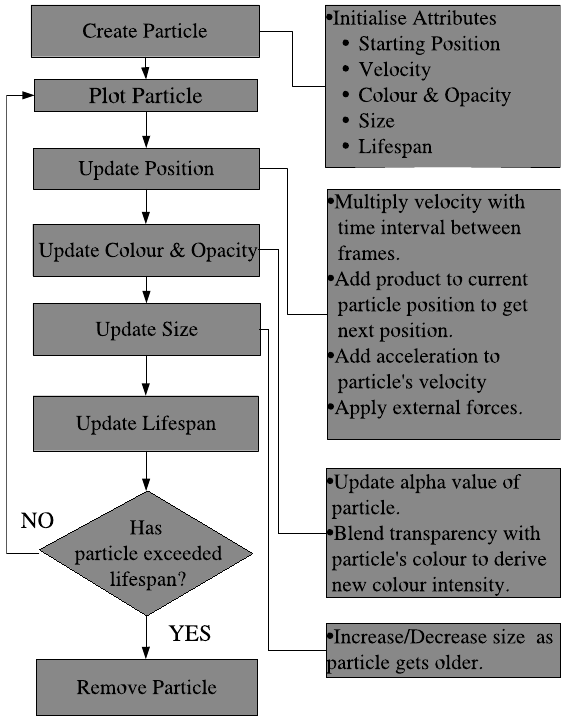
\includegraphics[width=0.7\textwidth]{algorithm}
    \caption{Схема обновления частиц в кадре, предложенная Вудхаузом
    в~\cite{Woodhouse}}%
    \label{fig:algorithm}
\end{figure}

Частицы создаются эмиттерами и затем вводятся в систему частиц.\break{}Эмиттеры
являются случайными точками, расположенными в рамках указанных границ. По факту,
можно считать эмиттеры статическими частицами.\break{}Эмиттеры обладают
различными характеристиками, которые вносят вклад в динамику частиц и общий
внешний вид модели огня. Ключевыми атрибутами эмиттеров являются их позиция,
скорость эмиссии частиц, начальный вектор эмиссии, динамический список частиц, и
энергия эмиттера.

Местоположение эмиттеров, определяет, где в пределах системы частиц будут
создаваться эмиттеры. В предложенной реализации эмиттеры создаются внутри круга,
который обозначает радиус огня. Эмиттеры также управляют скоростью эмиссии
частиц и преобладающим направлением эмиссии. Скорость эмиссии или скорость
горения определяет число частиц, которые испускает каждый эмиттер в момент
времени. Как видно на рисунке~\ref{fig:partLayers}
\begin{figure}[htb]
	\centering
	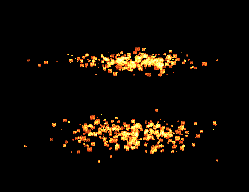
\includegraphics[width=0.4\textwidth]{partLayers}
    \caption{На картинке представлен эффект появления слоев, состоящих из частиц
    испущенных в один момент времени}%
    \label{fig:partLayers}
\end{figure}
частицы могут появляться в виде слоев на экране. Это происходит потому, что все
частицы с постоянной скоростью генерируются у основания эмиттера, вектора
движения частиц также совпадают. Для устранения данного недостатка можно при
генерации частиц добавить им случайное смещение вдоль оси $y$, также можно
добавить небольшие случайные смещения к начальным векторам скорости частиц.
Доработанная система демонстрирует более реалистичные результаты и представлена
на рисунке~\ref{fig:partLayersFix}.
\begin{figure}[htb]
	\centering
	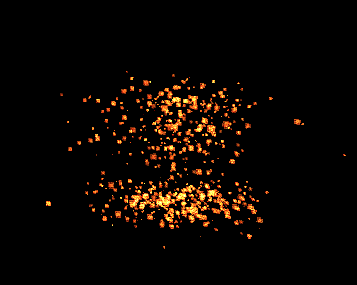
\includegraphics[width=0.4\textwidth]{partLayersFix}
    \caption{Уменьшение кластеризации частиц с помощью добавления случайных
    смещений}%
    \label{fig:partLayersFix}
\end{figure}
Эффект кластеризации может приводить к видимым разрывам в анимации из-за
существенного перепада количества частиц. Оптимальные значения для коэффициентов
смещения следует подбирать опытным путем.

Когда эмиттер создается ему присваивается случайное количество частиц, которые
хранятся в динамическом списке. Список изменяется при добавлении или удалении
частиц из системы. Как можно понять, производительность данного решения крайне
страдает из-за постоянных операций по управлению памятью. Решение данной
проблемы взято в~\cite{LearnOGL}. В данной работе предложено выделять память
заранее для каждого эмиттера, выделенная область ограничивает максимальное
количество частиц присутствующих в системе, которые были выделены одним
эмиттером. Для обновления атрибутов и дальнейшего рендеринга выбираются только
те частицы, которые имеют положительное значение оставшегося времени жизни. При
добавлении новой частицы в систему происходит поиск в списке уже неактивной
частицы и замена ее на новую.

Недостатками данной реализации являются:
\begin{enumerate}
    \item Необходимость определения максимального количества частиц в системе
    заранее. Это несет существенные затраты по памяти. Также при отсутствии
    свободных частиц происходит замена случайной частицы на новую, что может
    быть нежелательно.
    \item Высокая алгоритмическая сложность алгоритма поиска новой частицы.
    Алгоритм имеет линейную сложность ($O(n)$) в худшем случае. В алгоритме есть
    небольшая оптимизация. Алгоритм хранит индекс последней неиспользованной
    частицы, и пытается на следующем шаге начинать поиск с нее. Эта оптимизация
    слабо помогает при постоянном наличии большого числа частиц в системе.
    Если у частиц еще значительно варьируется время жизни --- практически всегда
    выполняется линейный поиск.
\end{enumerate}

Наибольшую проблему вызывал алгоритм обновления частиц. Он являлся бутылочным
горлышком системы. Для решения данной проблемы было разработано тривиальное, но
эффективное решение: в цикле обновления частиц индексы ''умерших'' частиц
помещаются в отдельный список. Данный список используется на следующем шаге
симуляции на этапе генерации новых частиц. Данное решение немного увеличило
затраты по памяти, однако позволило выполнять операцию поиска ''умерших'' частиц
за константное время ($O(1)$).

Вернемся к описанию эмиттеров. Энергия эмиттера определяет время жизни системы
частиц. Каждую итерацию энергия эмиттера уменьшается, пока не достигнет
минимального значения, обозначающего, что эмиттер иссяк. Иссякшие эмиттеры
убираются из системы вместе со всеми назначенными им частицами. Менеджер
эмиттеров содержит список всех эмиттеров в системе. Когда эмиттер создается, он
добавляется в динамический список. Менеджер эмиттеров каждую итерацию обновляет
все эмиттеры и удаляет иссякшие эмиттеры из системы. В
таблице~\ref{table:emitterAttribs} приведено описание всех атрибутов эмиттеров,
описанных на данный момент.
\begin{table}[htb]
\caption{Атрибуты эмиттера}%
\label{table:emitterAttribs}
\centering
\small
\begin{tabular}{| l | l |}
    \hline
    Атрибут & Описание \\
    \hline
    Позиция & Местоположение эмиттера в трехмерном пространстве \\
    Энергия & Время жизни эмиттера \\
    Скорость & Модуль начальной скорости испускаемых эмиттером частиц \\
    Направление & Единичный вектор, указывающий направление эмиссии частиц \\
    Радиус & Радиус эмиттера. Ограничивает область генерации частиц \\
    Список частиц & Динамически обновляемый список принадлежащих эмиттеру
    частиц \\
    \hline
\end{tabular}
\end{table}

В качестве структуры симулятора была выбрана схема, предложенная
в~\cite{Somasekaran2005UsingPS}. Общая структура симулятора представлена на
рисунке~\ref{fig:simStructure}.
\begin{figure}[htb]
	\centering
	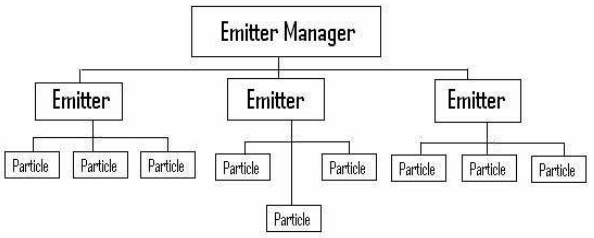
\includegraphics[width=\textwidth]{simStructure}
    \caption{Иерархия объектов, использованная в разработанном симуляторе}%
    \label{fig:simStructure}
\end{figure}

При описании структуры симулятора, достаточного внимание не было уделено
описанию частиц. Частицы являются ключевыми объектами в симуляции. Они имеют
такие атрибуты, как позицию, энергию (время жизни), цвет, скорость, ускорение и
размер.  Каждая частица появляется в системе недалеко от центра эмиттера, в
дальнейшем ее местоположение изменяется в течение всего времени жизни частицы.
Скорость частицы определяет ее следующее местоположение в системе. Для
улучшения визуального восприятия сцены, к частицам также применяется ускорение.
Как и эмиттеры, частицы также обладают атрибутом энергии, который определяет
время жизни частицы в системе. Когда частица исчерпала свою энергию, ее место
занимает новая, что позволяет оптимизировать операции по управлению памятью.
Цвет и размер частицы определяется на основе количества энергии частицы и играет
существенную роль в формировании визуального представления сцены. По мере
уменьшения энергии частицы ее размер, интенсивность цвета и прозрачность
уменьшаются. Это помогает создать эффект незаметного исчезновения частиц по
истечении их времени жизни. Краткий обзор всех атрибутов частиц представлен в
таблице~\ref{table:partAttribs}.
\begin{table}[htb]
\caption{Атрибуты частицы}%
\label{table:partAttribs}
\centering
\small
\begin{tabular}{| p{0.12\textwidth} | p{0.78\textwidth} |}
    \hline
    Атрибут & Описание \\
    \hline
    Позиция & Местоположение частицы в трехмерном пространстве \\
    Скорость & Вектор скорости частицы \\
    Ускорение & Вектор ускорения частицы \\
    Энергия & Представляет оставшееся время жизни частицы \\
    Цвет & Цвет частицы. Интенсивность и прозрачность уменьшаются по мере
    старения частицы \\
    Размер & Размер частицы. Размер частицы уменьшается по мере старения частицы \\
    \hline
\end{tabular}
\end{table}

Первый прототип системы представлен на рисунке~\ref{fig:firstProto}.
\begin{figure}[htb]
	\centering
    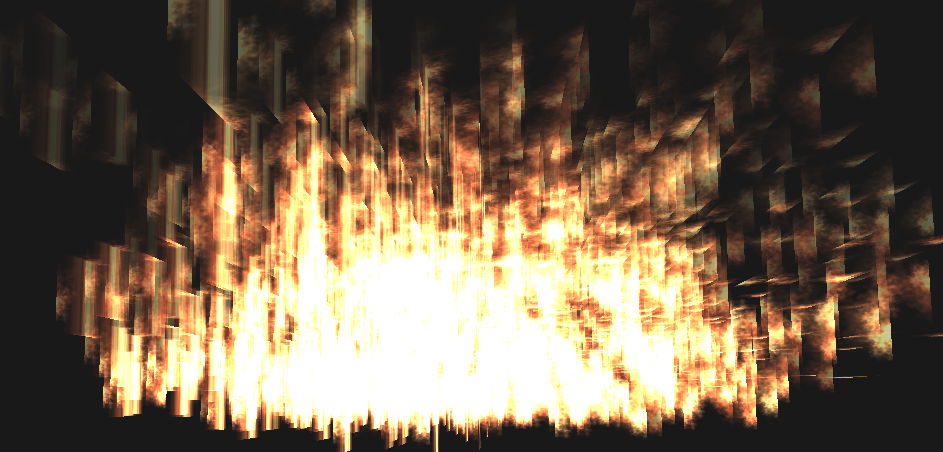
\includegraphics[width=\textwidth]{firstProto}
    \caption{Первый прототип системы}%
    \label{fig:firstProto}
\end{figure}
Данный прототип страдал от множества недостатков:
\begin{enumerate}
    \item Высокая загрузка ГП. Несмотря на сравнительно небольшое количество
        объектов загрузка ГП достигала 85\%. При этом в системе находилось всего
        лишь 500 частиц. Каждый кадр генерировалось по 20 частиц.
    \item Проблемы с текстурами. Ошибка с наложением текстур была исправлена в
        следующих версиях.
    \item Отсутствие должной анимации частиц. Все частицы летят строго в
        направлении эмиссии. Созданию анимации пламени будет посвящен отдельный
        раздел.
\end{enumerate}

Ключевой проблемой на данной стадии являлась чрезмерная загрузка ГП. Для
устранения этой проблемы была задействована техника инстансинга. Идеей данного
метода является уменьшение количества вызовов к ГП. Более подробно
эта техника описана в~\cite{OGLSuperbible,LearnOGL}. Данная техника хорошо
подходит для рендеринга множества однородных объектов, какими и являются
частицы. Вместо того, чтобы в цикле выставлять атрибуты частицы и вызывать вызов
для отрисовки, атрибуты всех частиц записываются в массивы. Для рендеринга всех
частиц требуется лишь вызвать функцию \texttt{glDrawArraysInstanced}. Реализация
данной техники позволило увеличить количество частиц в системе до 5000,
количество частиц создаваемых за кадр --- до 750. При этом нагрузка на ГП
снизилась до 28\%. Модифицированная система представлена на
рисунке~\ref{fig:proto2}.
\begin{figure}[htb]
	\centering
    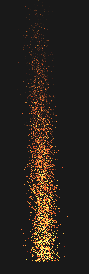
\includegraphics[height=8cm]{proto2}
    \caption{Использование инстансинга для отрисовки частиц}%
    \label{fig:proto2}
\end{figure}

Увеличение максимального числа частиц и уменьшение их размера положительно
скажется на реалистичности анимации. Однако, оптимизация работы ГП
продемонстрировала недостатки алгоритмов, работающих на ЦП. Загрузка ЦП
достигала 100\% (симуляция выполняется в один поток).

Для решения данной проблемы был использована оптимизация алгоритма обновления
частиц, описанная выше в данном разделе. Данная оптимизация позволила снизить
среднюю загрузку ЦП до 18\%, что позволило выполнять симуляцию с частотой 60
кадров / секунду. Изменения можно увидеть на рисунке~\ref{fig:proto3}.
\begin{figure}[htb]
	\centering
    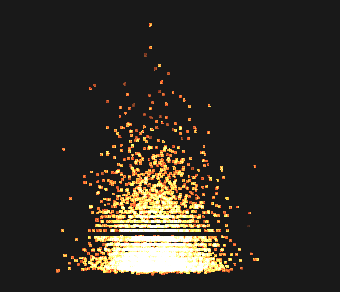
\includegraphics[width=0.4\textwidth]{proto3}
    \caption{Система, основанная на новом алгоритме поиска ''мертвых'' частиц}%
    \label{fig:proto3}
\end{figure}

Изменение высоты пламени и скорости движения частиц вызваны изменением алгоритма
поиска ''мертвых'' частиц. В прошлой версии алгоритма при отсутствии свободных
частиц добавления новой частицы не происходило, в новой версии происходит замена
случайной частицы при неудаче. В продемонстрированном примере часто происходит
удаление случайных частиц и замена их на новые. Из-за данного эффекта
увеличилась плотность частиц у основания пламени, визуально увеличилась скорость
частиц. Удаление случайных частиц позволило устранить эффект непрерывного столба
пламени, наблюдаемый на рисунке~\ref{fig:proto2}. Данный эффект положительно
сказался на визуальном восприятии сцены и будет использован в дальнейшем.

Дальнейшие улучшения были связаны увеличением стохастичности симуляции. К
значениям многих атрибутов были добавлены случайные смещения, что позволило
уменьшить количество статических элементов симуляции. Система с внесенными
оптимизациями и улучшениями представлена на рисунке~\ref{fig:proto4}.
\begin{figure}[htb]
	\centering
    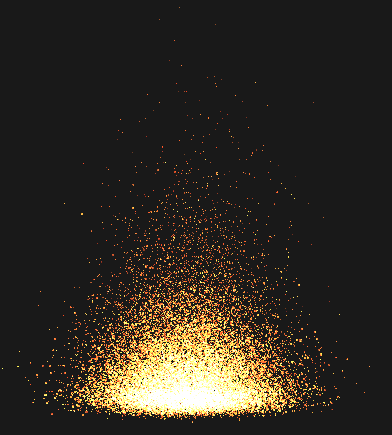
\includegraphics[width=0.4\textwidth]{proto4}
    \caption{Использование стохастических эффектов в симуляции}%
    \label{fig:proto4}
\end{figure}
Однако, наиболее заметным недостатком данной системы является отсутствие
анимации. Решение, использованное для анимации системы будет описано в следующем
разделе.

\section{Анимация пламени}

В ходе исследования различных алгоритмов для анимации огня, был проведен обзор
нескольких различных подходов, описание которых можно найти в
главе~\ref{chap:lit_review}. В общем случае, в момент времени $(t)$ новое
положение частицы зависит от ее скорости $\vec{v}(t)$, ускорения $\vec{a}$, и интервала
времени между кадрами $\Delta t$. Как было замечено ранее, начальный вектор
скорость частицы определяется вектором эмиссии конкретного эмиттера. Для расчета
следующего положения частицы $\vec{p}(t + \Delta{t})$, используется следующие
уравнения (\ref{eq:position},~\ref{eq:velocity}).
\begin{equation}
  \label{eq:position}
  \vec{p}(t + \Delta{t}) = \vec{p}(t) + \vec{v}(t) \cdot \Delta{t}
\end{equation}
\vspace{-1em}
\begin{equation}
  \label{eq:velocity}
  \vec{v}(t + \Delta{t}) = \vec{v}(t) + \vec{a}
\end{equation}
\begin{explanationx}
    \item [где] $\vec{p}(t + \Delta{t})$ --- координаты частицы в следующий
        момент времени;
    \item $\vec{p}(t)$ --- текущие координаты частицы;
    \item $\vec{v}(t)$ --- скорость частицы в текущий момент времени;
    \item $\Delta{t}$ --- величина временного интервала между текущим и прошлым кадром;
    \item $\vec{v}(t + \Delta{t})$ --- скорость частицы в следующий момент времени;
    \item $\vec{a}$ --- текущее ускорение частицы.
\end{explanationx}

Как видно из уравнений выше, движение частиц в системе является равноускоренным.
Частицы немного ускоряются по мере их движения. Для данной симуляции была
эмпирически подобрана величина ускорения, вычисляемая по следующей формуле
(\ref{eq:accelearation}).
\begin{equation}
  \label{eq:accelearation}
  \vec{a} = 0.02 \cdot \vec{\text{v}_\text{0}}
\end{equation}
\begin{explanationx}
    \item [где] $\vec{a}$ --- ускорение частицы;
    \item $\vec{\text{v}_\text{0}}$ --- начальная скорость частицы.
\end{explanationx}

Как можно заметить, описанные выше уравнения описывают движение частиц как
равноускоренное прямолинейное движение. Однако, как было описано в
разделе~\ref{section:firePerception}, воздействующие на огонь силы создают более
сложное движение частиц пламени. Важным отличием реального огня, от описанной
выше модели, является постоянное движение и изменение формы языков пламени. В
статье~\cite{Harris} Том Харрис%TODO
